% !TeX root = ../../main.tex
\question{پیاده‌سازی مدل خودرمزگذار متغیر (VAE) و تحلیل تجربی توزیع‌های پیشین}
\label{sec:question2}

در این بخش، پیاده‌سازی کامل و ارزیابی تجربی مدل خودرمزگذار متغیر (\lr{Variational Autoencoder - VAE}) بر روی یک مجموعه داده ساخت‌یافته ۲۰‌بعدی گزارش می‌شود. هدف اصلی، بررسی اثرات هندسی و آماری انتخاب توزیع پیشین (\lr{Prior Distribution}) بر روی کیفیت بازسازی، دقت داده‌های تولیدی، و ساختار فضای نهفته است. در ادامه، چهار مدل با توزیع‌های پیشین متفاوت (گاوسی استاندارد، ترکیب گاوسی ۸‌تایی ثابت، ترکیب گاوسی ۸‌تایی یادگیرنده، و ترکیب گاوسی ۴‌تایی یادگیرنده) به صورت جامع مقایسه و تحلیل می‌شوند.

% =========================================================================
% ۱. معماری و آموزش
% =========================================================================
\subsection{معماری شبکه، تابع هزینه و دینامیک آموزش}
\label{sec:q2-arch}

\textbf{تولید داده‌ها و ویژگی‌ها:} مجموعه داده شامل ۹۶۰۰ نمونه ۲۰‌بعدی است که از ۸ خوشه دایره‌ای در یک فضای منبع دوبعدی منشأ می‌گیرند و از طریق نگاشت‌های غیرخطی مثلثاتی، چندجمله‌ای و اغتشاش نویز گاوسی همسانگرد با انحراف معیار $0.07$ تولید شده‌اند. داده‌ها به سه بخش آموزش (۷۰٪ معادل ۶۷۲۰ نمونه)، اعتبارسنجی (۱۵٪ معادل ۱۴۴۰ نمونه) و آزمون (۱۵٪ معادل ۱۴۴۰ نمونه) افراز شده و بر اساس میانگین و انحراف معیار بخش آموزش استانداردسازی شده‌اند.

\textbf{معماری رمزگذار و رمزگشا:} مطابق صورت تمرین، ساختار شبکه‌ها به صورت زیر طراحی شده است:
\begin{itemize}
  \item \textbf{رمزگذار (\lr{Encoder}):} شبکه پیش‌خور دو لایه پنهان با ابعاد $20 \to 128 \to 128 \to 2$ با فعال‌ساز \lr{ReLU} که پارامترهای پسین متغیر یعنی بردار میانگین $\mu_\phi(x)$ و لگاریتم واریانس قطری $\log\sigma_\phi^2(x)$ را در فضای نهفته دوبعدی تولید می‌کند. نمونه‌برداری از فضای نهفته با ترفند بازپارامتری‌سازی انجام می‌شود: $z = \mu_\phi(x) + \sigma_\phi(x) \odot \epsilon$ با $\epsilon \sim \mathcal{N}(0, I_2)$.
  \item \textbf{رمزگشا (\lr{Decoder}):} شبکه پیش‌خور دو لایه پنهان با ابعاد $2 \to 128 \to 128 \to 20$ با فعال‌ساز \lr{ReLU} که میانگین بازسازی $\mu_\theta(z)$ را برآورد می‌نماید.
\end{itemize}

\textbf{تابع درست‌نمایی و بازسازی:} با فرض درست‌نمایی گاوسی همسانگرد با واریانس ثابت $\sigma_x^2 = 0.30^2 = 0.09$، تابع اتلاف منفی لگاریتم درست‌نمایی (\lr{NLL}) برای بعد $D=20$ به فرم تحلیلی زیر محاسبه می‌شود:
\begin{equation}
  \mathcal{L}_{\text{recon}}(x, \mu_\theta(z)) = \frac{1}{2\sigma_x^2} \|x - \mu_\theta(z)\|^2 + \frac{D}{2}\log(2\pi\sigma_x^2) = \frac{1}{0.18} \|x - \mu_\theta(z)\|^2 - 5.7006
  \label{eq:recon-nll}
\end{equation}
ضریب وزنی $\frac{1}{0.18} \approx 5.5556$ نقش حیاتی در ایجاد تعادل مناسب میان بازسازی داده و منظم‌سازی واگرایی \lr{KL} ایفا می‌کند.

\textbf{واگرایی کولبک-لایبلر (\lr{KL Divergence}):}
برای مدل A (پیشین گاوسی استاندارد $p(z) = \mathcal{N}(0, I_2)$)، واگرایی به صورت تحلیلی و بسته محاسبه می‌شود:
\begin{equation}
  D_{\text{KL}}\!\left(q_\phi(z\mid x)\,\|\,\mathcal{N}(0, I)\right) = -\frac{1}{2}\sum_{j=1}^2 \left(1 + \log\sigma_j^2(x) - \mu_j^2(x) - \sigma_j^2(x)\right)
\end{equation}
برای مدل‌های مبتنی بر ترکیب گاوسی (B، C، و D)، واگرایی فاقد فرم تحلیلی بسته است و با برآوردگر مونت‌کارلو تک‌نمونه‌ای پایدار با تابع \lr{logsumexp} پیاده‌سازی شده است:
\begin{equation}
  D_{\text{KL}}\!\left(q_\phi(z\mid x)\,\|\,p(z)\right) \approx \log q_\phi(z\mid x) - \log p(z), \quad z \sim q_\phi(z\mid x)
\end{equation}
که در آن برای هر مدل ترکیب گاوسی با $K$ مؤلفه و وزن‌های یکنواخت $\pi_k = \frac{1}{K}$:
\begin{equation}
  \log p(z) = \mathop{\mathrm{logsumexp}}_{k=1}^K \left[ -\log K - \log(2\pi) - \sum_{j=1}^2 \log\sigma_{kj} - \frac{1}{2}\sum_{j=1}^2 \frac{(z_j - \mu_{kj})^2}{\sigma_{kj}^2} \right]
\end{equation}

\textbf{پیکربندی آموزش و توقف زودهنگام:} کلیه مدل‌ها با بهینه‌ساز \lr{Adam}، نرخ یادگیری $10^{-3}$، اندازه دسته ۶۴، و مکانیزم توقف زودهنگام با شکیبایی ۱۵ دوره (\lr{Patience}) بر روی اتلاف کل اعتبارسنجی آموزش داده شدند. روند همگرایی منحنی‌های اتلاف در شکل~\ref{fig:learning-curves} نشان داده شده است. بهترین دوره‌ها به ترتیب عبارتند از: مدل A در دوره ۹۹، مدل B در دوره ۹۷، مدل C در دوره ۱۰۰، و مدل D در دوره ۹۹.

\begin{figure}[htbp]
  \centering
  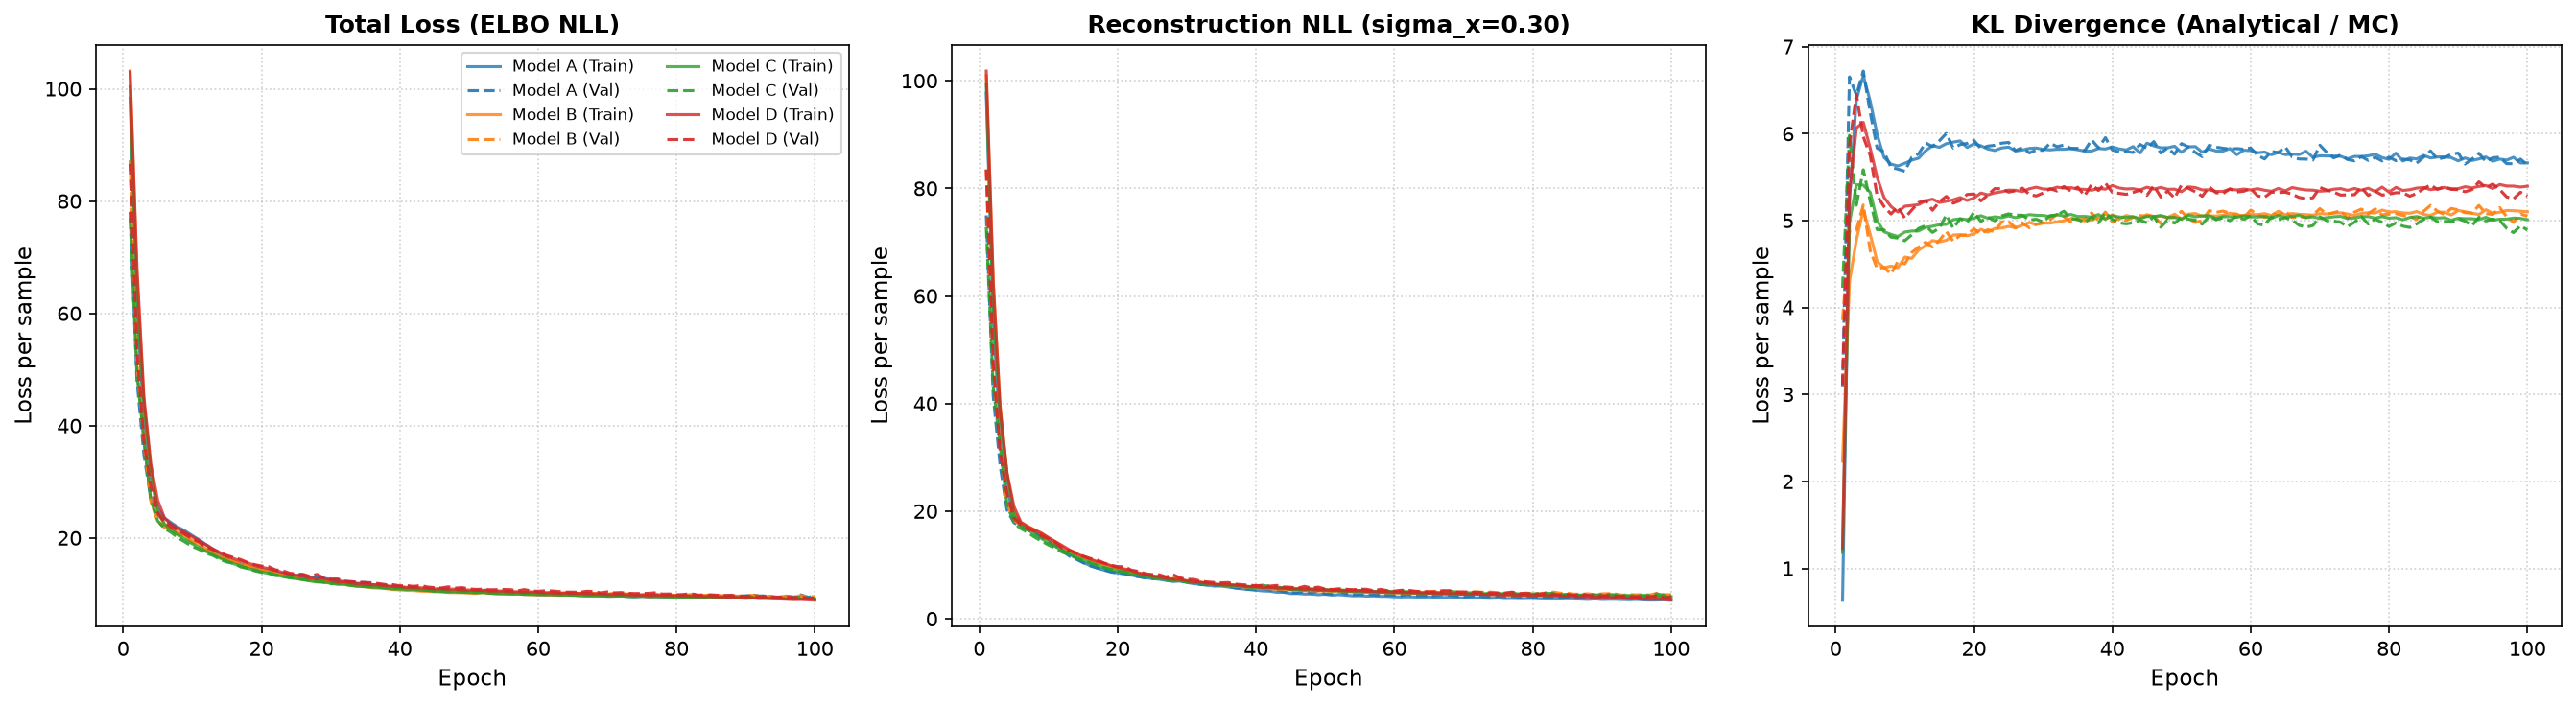
\includegraphics[width=0.92\linewidth]{problems/question2/results/learning_curves_all_models.png}
  \caption{منحنی‌های آموزش و اعتبارسنجی اتلاف کل، اتلاف بازسازی و واگرایی \lr{KL} برای هر چهار مدل.}
  \label{fig:learning-curves}
\end{figure}

% =========================================================================
% ۲. بازسازی و PCA
% =========================================================================
\subsection{تحلیل کیفیت بازسازی و توزیع داده‌های تولیدی در فضای PCA}
\label{sec:q2-recon-pca}

\textbf{کیفیت بازسازی بر روی داده‌های آزمون:} ارزیابی بازسازی منحصراً بر روی ۱۴۴۰ نمونه بخش آزمون و با استفاده از میانگین پسین تعیینی $\mu_\phi(x)$ بدون اضافه کردن نویز مشاهده انجام شد. مطابق جدول~\ref{tab:master-evaluation}، کمترین خطای بازسازی به ترتیب متعلق به مدل D (با خطای هر عنصر $0.07764$) و مدل A (با خطای $0.07802$) است، در حالی که مدل‌های C ($0.08221$) و B ($0.08246$) دارای خطای بازسازی اندکی بالاتر (حدود ۶٪ بیشتر) هستند. علت فیزیکی این پدیده آن است که توزیع‌های پیشین تک‌مؤلفه‌ای یا با تعداد مؤلفه اندک، قید هندسی کمتری بر چیدمان کدهای نهفته تحمیل کرده و به رمزگذار اجازه می‌دهند کدهای نهفته را پیوسته و آزادانه به گونه‌ای تنظیم کند که خطای بازسازی به حداقل برسد. برعکس، پیشین‌های ۸‌مؤلفه‌ای، پسین را مقید به تمرکز حول ۸ مد گسسته می‌کنند که موجب یک تنش ساختاری جزئی میان بهینه‌سازی بازسازی و انطباق با پیشین می‌شود.

\textbf{تولید نمونه و نگاشت در فضای \lr{PCA}:} برای هر مدل، ۲۰۰۰ نمونه مستقل از پیشین $z \sim p(z)$ استخراج و توسط رمزگشا بازسازی شدند. به منظور پرهیز از نشت اطلاعات، این نمونه‌ها و همچنین داده‌های آزمون بر روی فضای \lr{PCA} دوبعدی که منحصراً بر روی داده‌های آموزش فیت شده بود نگاشت شدند (شکل~\ref{fig:pca-all-grid}). 

\begin{figure}[htbp]
  \centering
  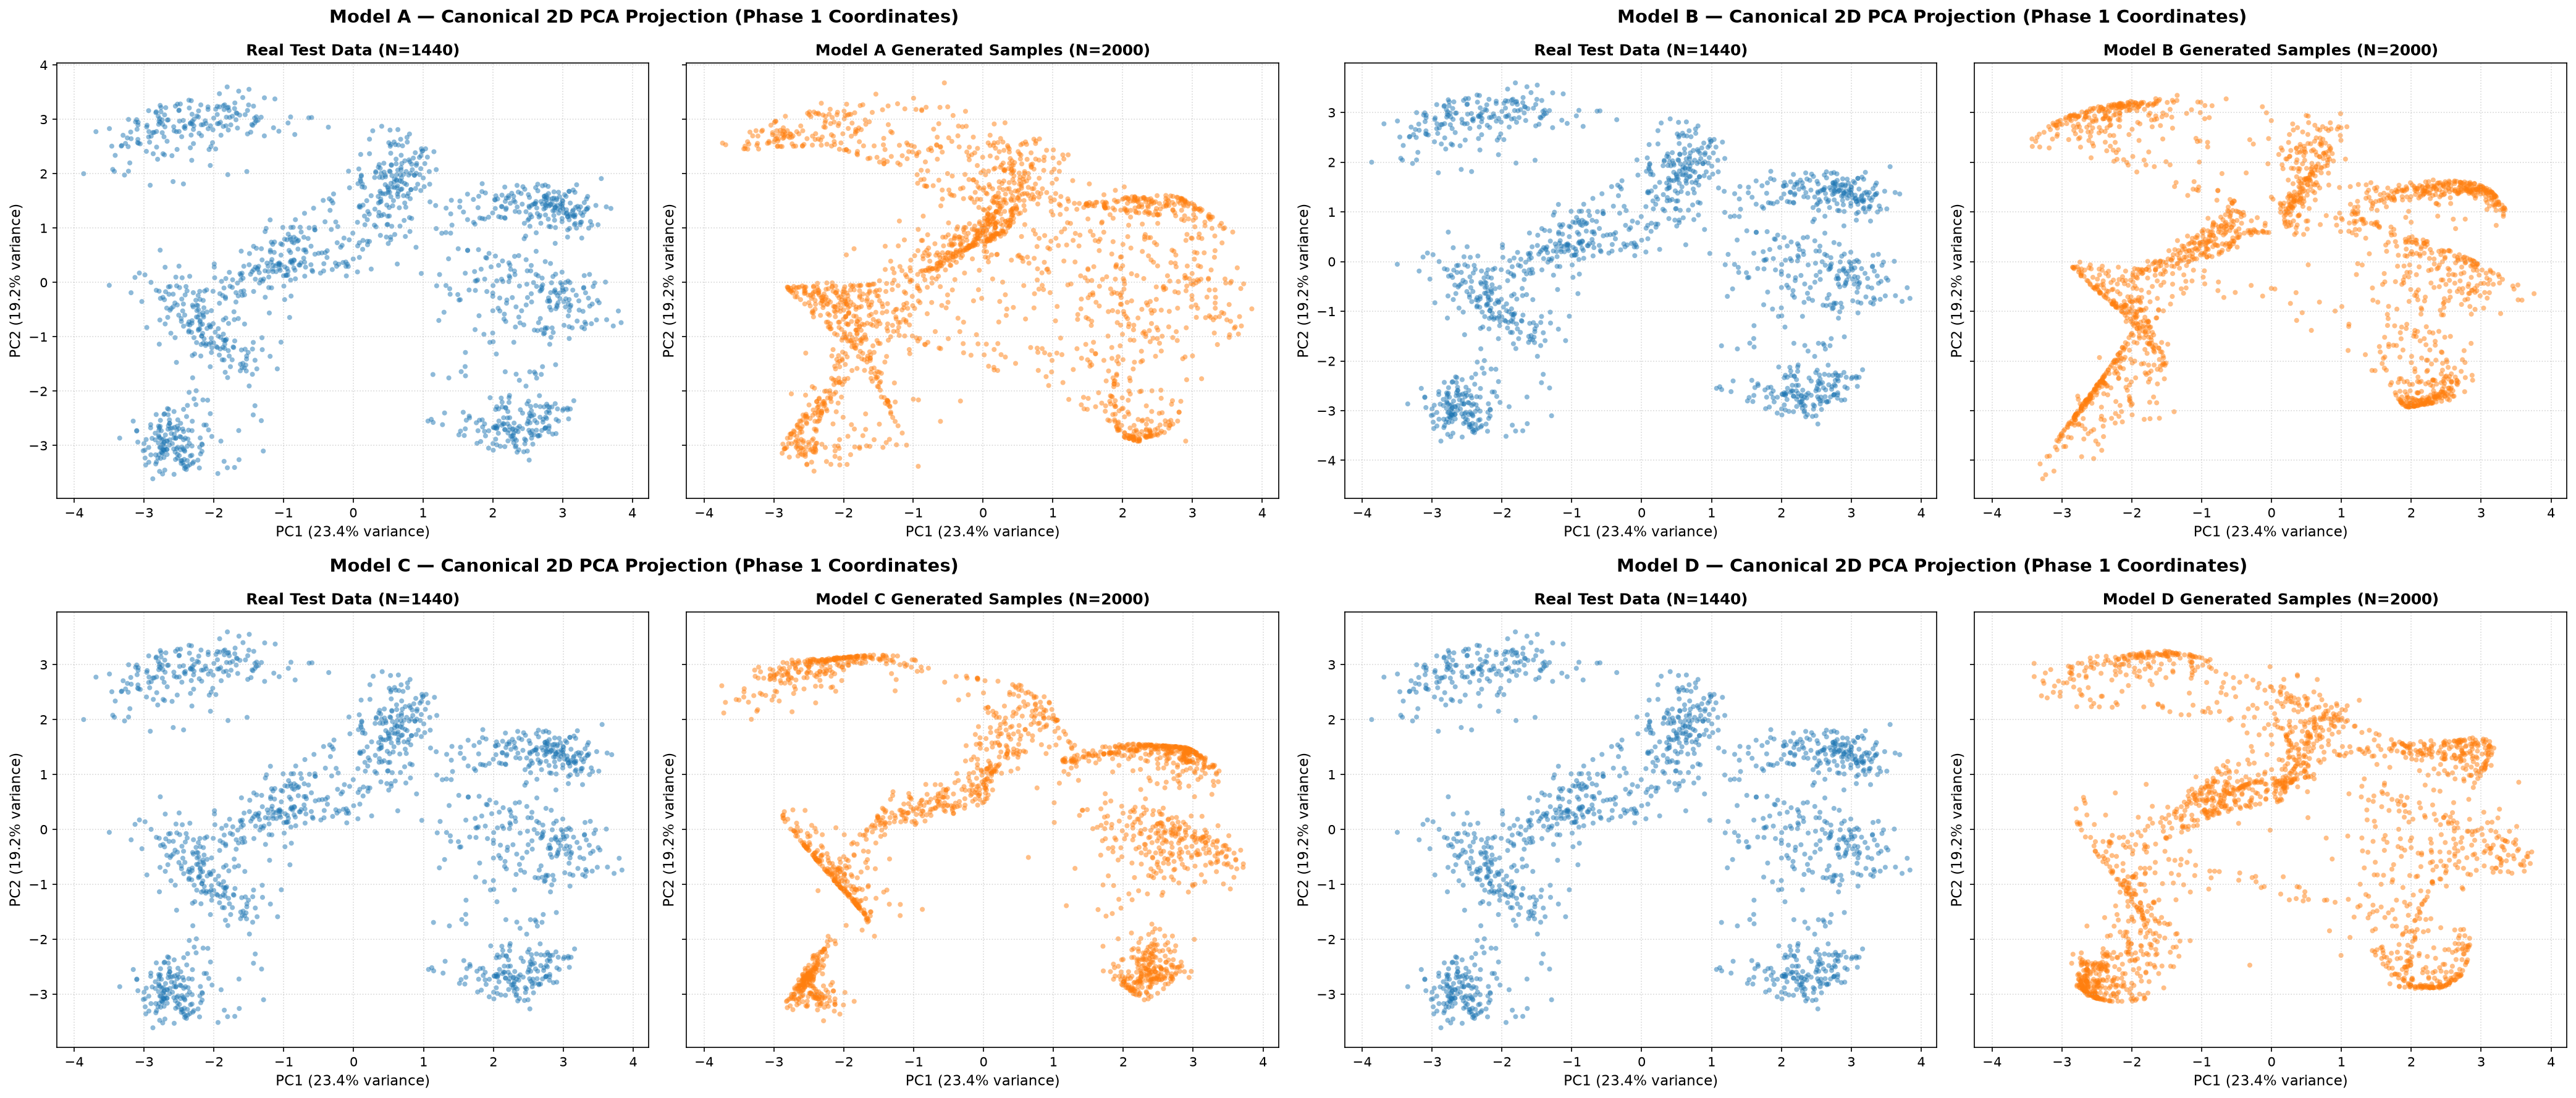
\includegraphics[width=0.95\linewidth]{problems/question2/results/pca_test_vs_generated_all_grid.png}
  \caption{تصویر دوبعدی \lr{PCA} از نمونه‌های واقعی آزمون (آبی) در برابر نمونه‌های تولیدشده از پیشین (قرمز) برای هر چهار مدل.}
  \label{fig:pca-all-grid}
\end{figure}

تحلیل تصاویر شکل~\ref{fig:pca-all-grid} نکات عمیقی را آشکار می‌سازد:
\begin{enumerate}
  \item \textbf{مدل A (پیشین گاوسی استاندارد):} به دلیل پیوستگی و تک‌مدی بودن پیشین $\mathcal{N}(0, I_2)$، نمونه‌های تولیدی در فضای میانی و مرکز خوشه‌ها (جایی که در داده‌های واقعی تهی است) پراکنده شده‌اند و پدیده \lr{Mode Bridging} و تولید نمونه‌های نامعتبر بین‌خوشه‌ای به وضوح رخ داده است.
  \item \textbf{مدل B (پیشین ۸‌تایی ثابت):} انطباق هندسی فوق‌العاده‌ای با خوشه‌های واقعی آزمون دارد و مرزهای خوشه‌ها کاملاً مجزا و تفکیک‌شده بازتولید شده‌اند.
  \item \textbf{مدل C (پیشین ۸‌تایی یادگیرنده):} تمام ۸ مد اصلی را با تراکم بالا پوشش داده و فاقد نمونه‌های زائد در مرکز است.
  \item \textbf{مدل D (پیشین ۴‌تایی یادگیرنده):} به علت کمبود مؤلفه‌ها ($K=4$ در برابر ۸ خوشه واقعی)، هر مؤلفه ناگزیر دو خوشه مجاور را پوشش داده و خوشه‌ها به صورت دوتایی به هم متصل شده‌اند.
\end{enumerate}

% =========================================================================
% ۳. فضای نهفته و تحلیل مؤلفه‌ها
% =========================================================================
\subsection{تحلیل هندسه فضای نهفته و میزان بهره‌برداری از مؤلفه‌های پیشین}
\label{sec:q2-latent}

در شکل~\ref{fig:latent-all-grid}، توزیع کدهای نهفته داده‌های آزمون در کنار خطوط تراز و مؤلفه‌های توزیع پیشین نمایش داده شده است.

\begin{figure}[htbp]
  \centering
  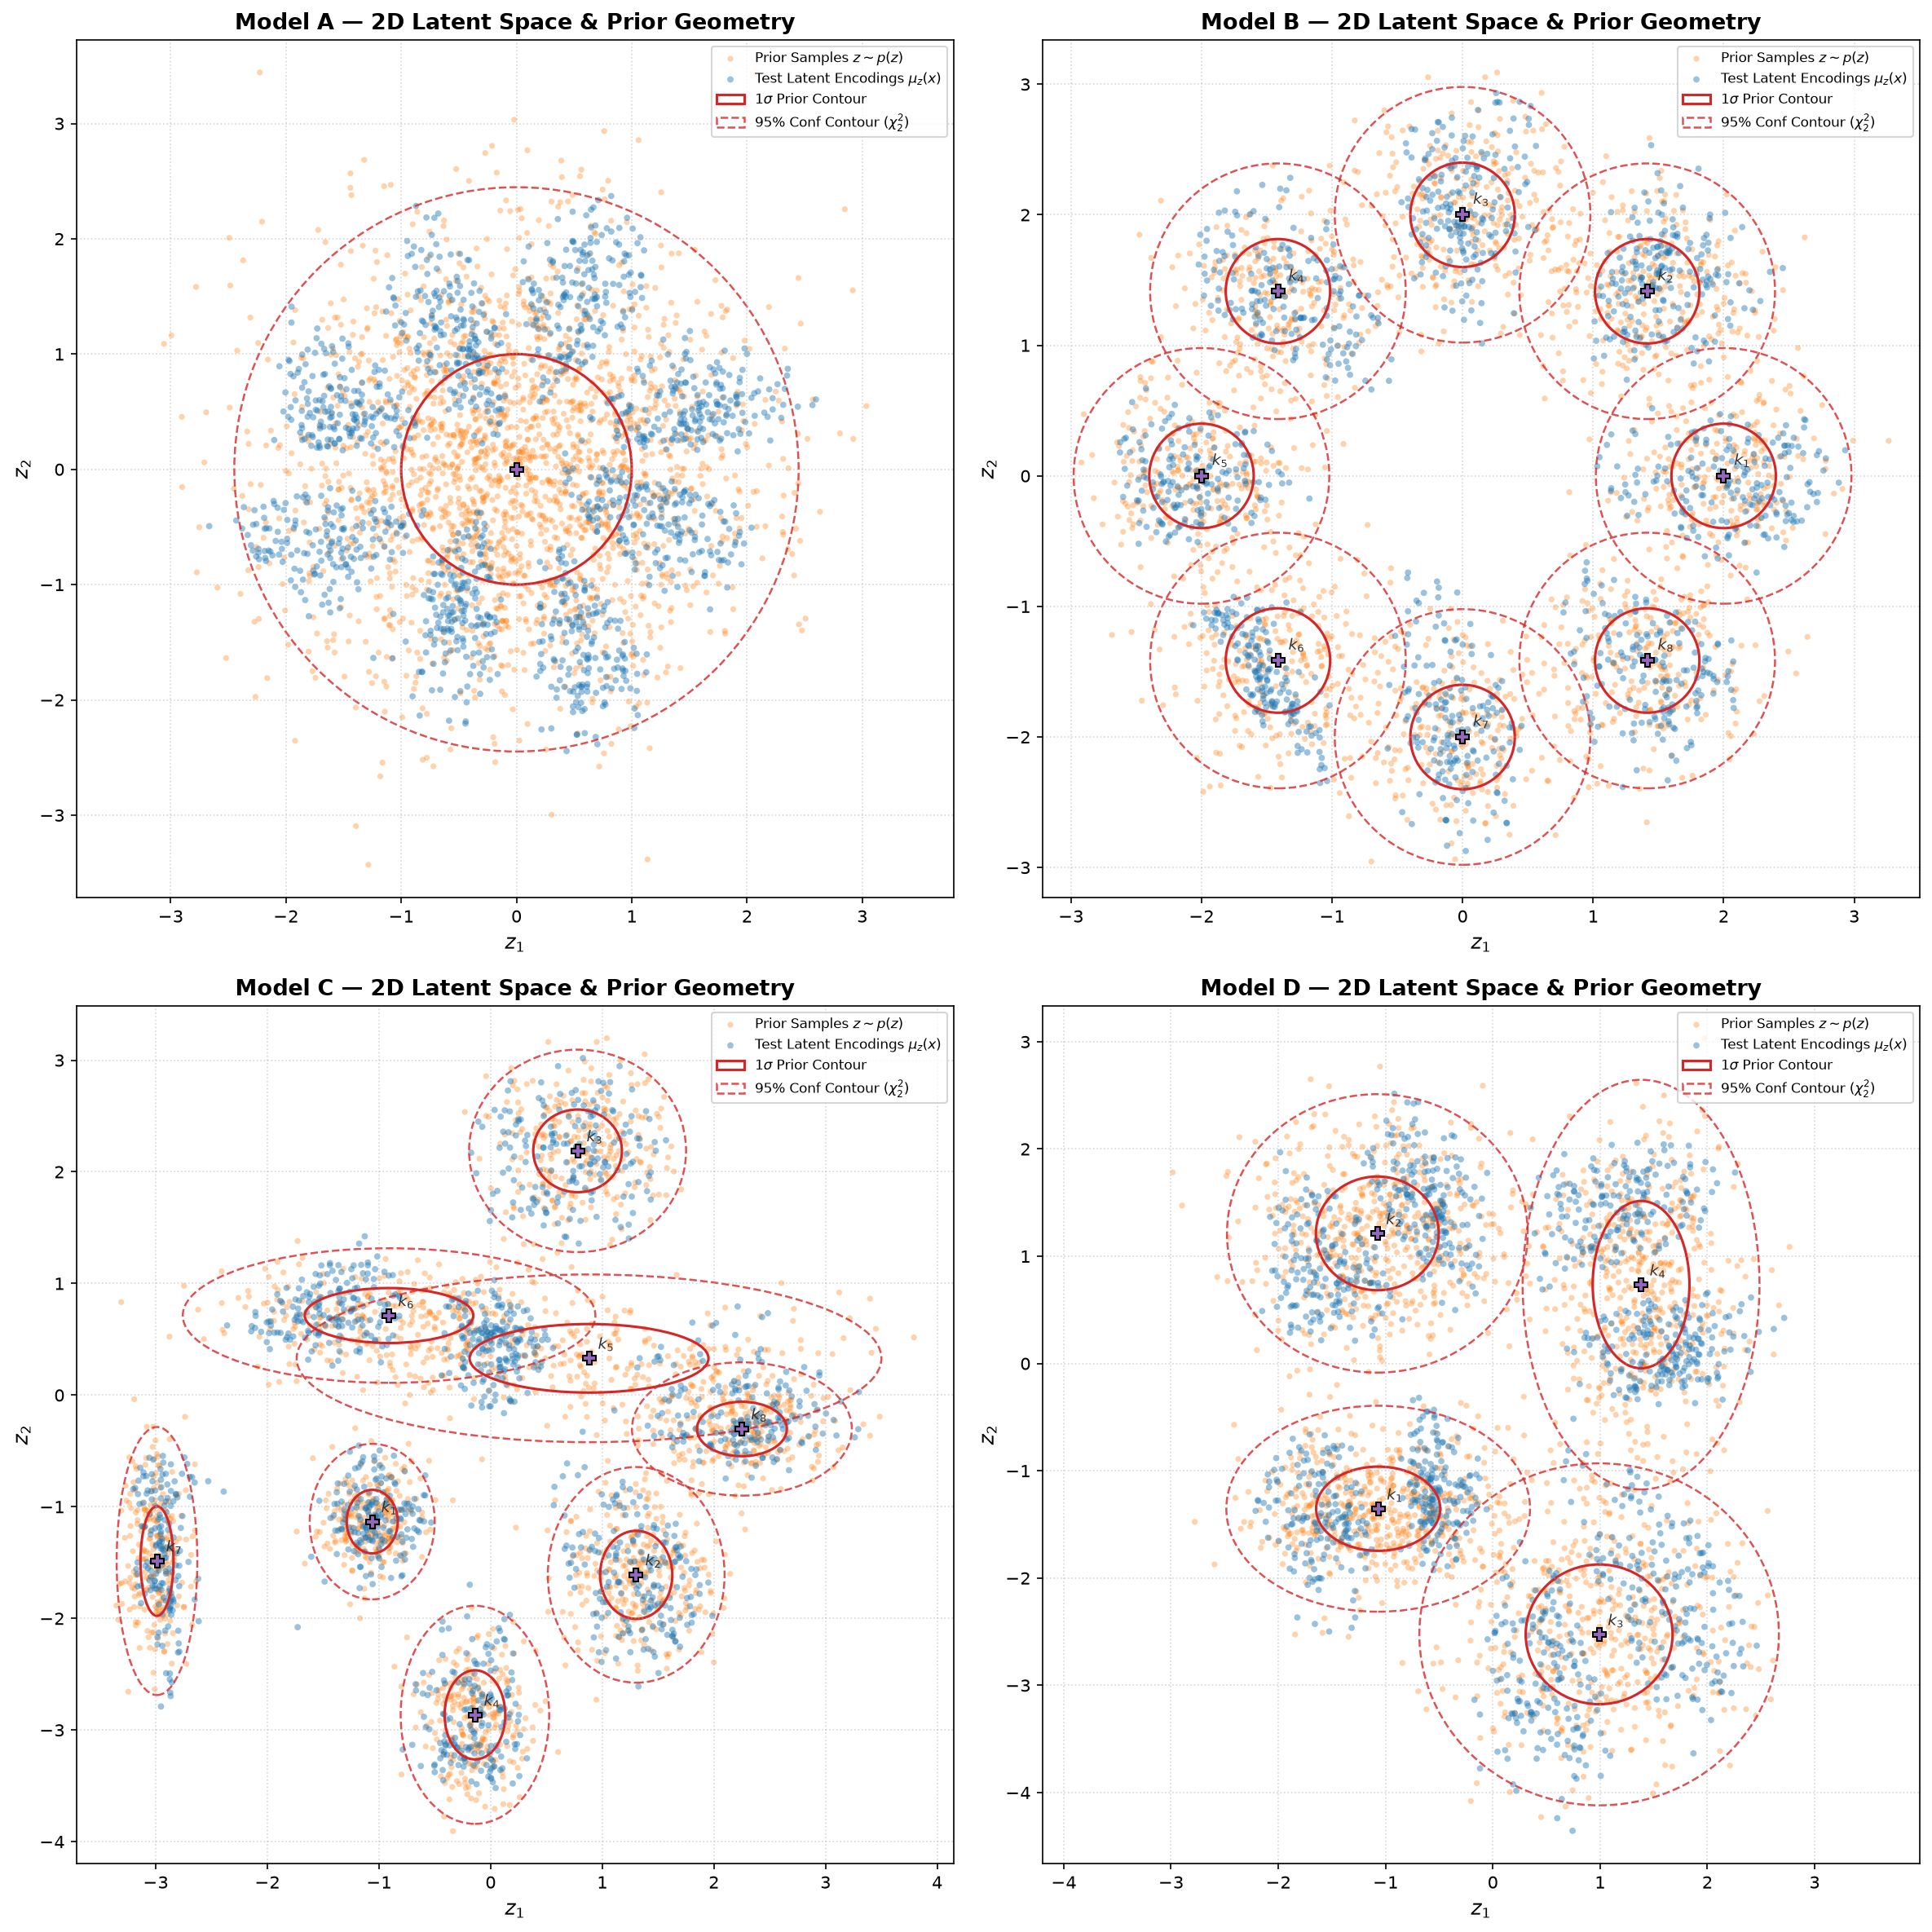
\includegraphics[width=0.88\linewidth]{problems/question2/results/latent_space_all_grid.png}
  \caption{نمایش فضای نهفته دوبعدی: کدهای نهفته آزمون به همراه کانتورها و مراکز مؤلفه‌های پیشین برای مدل‌های A، B، C و D.}
  \label{fig:latent-all-grid}
\end{figure}

\textbf{پاسخ به سوال تحلیلی ۴ (میزان استفاده از مؤلفه‌ها بر اساس چگالی بیشینه):}
برای مدل‌های ترکیب گاوسی، میزان بهره‌برداری از مؤلفه‌ها بر اساس دو شاخص سنجیده شد:
۱) نسبت تخصیص سخت (\lr{Hard Assignment}) با انتخاب مؤلفه دارای بیشترین چگالی $k^*(z) = \arg\max_k \mathcal{N}(z; \mu_k, \Sigma_k)$، و
۲) میانگین مسئولیت پسین (\lr{Mean Posterior Responsibility}) $\gamma_k(z) = \frac{\pi_k \mathcal{N}(z; \mu_k, \Sigma_k)}{\sum_j \pi_j \mathcal{N}(z; \mu_j, \Sigma_j)}$.
نتایج استخراج‌شده از آزمایش به شرح زیر است:
\begin{itemize}
  \item \textbf{مدل B (۸ مؤلفه ثابت):} تخصیص سخت بین ۱۱.۷۴٪ تا ۱۳.۶۸٪ و میانگین مسئولیت بین ۱۱.۷۶٪ تا ۱۳.۷۱٪ کاملاً متعادل است (مقدار ایده‌آل یکنواخت ۱۲.۵٪ است). هیچ‌یک از مؤلفه‌ها دچار زوال (\lr{Component Collapse}) نشده‌اند.
  \item \textbf{مدل C (۸ مؤلفه یادگیرنده):} تمامی ۸ مؤلفه فعال و در حال استفاده هستند (سهم تخصیص سخت بین ۱۰.۰۰٪ تا ۱۷.۳۶٪ و میانگین مسئولیت بین ۱۰.۸۸٪ تا ۱۶.۸۵٪). مراکز یادگرفته‌شده در فضای نهفته در شعاع‌های مختلف حول مبدا توزیع شده و هندسه چندخوشه‌ای را با موفقیت تفکیک کرده‌اند.
  \item \textbf{مدل D (۴ مؤلفه یادگیرنده):} هر ۴ مؤلفه با تعادل بالا (سهم تخصیص سخت بین ۲۳.۷۵٪ تا ۲۶.۶۷٪ و میانگین مسئولیت بین ۲۳.۵۱٪ تا ۲۶.۶۷٪ نسبت به سهم یکنواخت ۲۵٪) مورد استفاده قرار گرفته‌اند.
\end{itemize}

% =========================================================================
% ۴. ارزیابی کمی
% =========================================================================
\subsection{ارزیابی کمی: معیارهای MMD، پوشش خوشه‌ها و پاسخ به سوالات ۱ تا ۳}
\label{sec:q2-quant}

جدول~\ref{tab:master-evaluation} نتایج جامع کلیه معیارهای ارزیابی را برای هر چهار مدل خلاصه می‌کند.

\begin{table}[htbp]
  \centering
  \caption{جدول مقایسه جامع معیارهای ارزیابی در هر چهار مدل VAE.}
  \label{tab:master-evaluation}
  \resizebox{\textwidth}{!}{%
  \begin{tabular}{lcccccccc}
    \toprule
    \rowcolor{dgmAccent}
    \textcolor{white}{\bfseries مدل} &
    \textcolor{white}{\bfseries نوع پیشین} &
    \textcolor{white}{\bfseries بهترین دوره} &
    \textcolor{white}{\bfseries MSE هر عنصر} &
    \textcolor{white}{\bfseries MSE کل نمونه} &
    \textcolor{white}{\bfseries $\text{MMD}^2$ داده} &
    \textcolor{white}{\bfseries $\text{MMD}^2$ نهان} &
    \textcolor{white}{\bfseries نرخ اعتبار (\%)} &
    \textcolor{white}{\bfseries پوشش خوشه‌ها} \\
    \midrule
    \rowcolor{dgmLight}
    مدل A & گاوسی استاندارد & ۹۹ & ۰.۰۷۸۰۲ & ۱.۵۶۰۴ & ۰.۰۰۶۶۳۷ & ۰.۰۱۱۱۶۱ & ۸۰.۱۰٪ & ۸ از ۸ \\
    مدل B & ۸ مؤلفه ثابت ($r=2$) & ۹۷ & ۰.۰۸۲۴۶ & ۱.۶۴۹۲ & \textbf{۰.۰۰۰۹۴۳} & \textbf{-۰.۰۰۰۳۷۲} & ۹۵.۲۵٪ & ۸ از ۸ \\
    \rowcolor{dgmLight}
    مدل C & ۸ مؤلفه یادگیرنده & ۱۰۰ & ۰.۰۸۲۲۱ & ۱.۶۴۴۲ & ۰.۰۰۱۹۹۵ & ۰.۰۰۳۲۱۴ & \textbf{۹۵.۶۵٪} & ۸ از ۸ \\
    مدل D & ۴ مؤلفه یادگیرنده & ۹۹ & \textbf{۰.۰۷۷۶۴} & \textbf{۱.۵۵۲۸} & ۰.۰۰۱۸۲۵ & ۰.۰۰۰۵۸۸ & ۹۳.۰۰٪ & ۸ از ۸ \\
    \bottomrule
  \end{tabular}%
  }
\end{table}

\textbf{پاسخ به سوال تحلیلی ۱ (رتبه‌بندی مدل‌ها از نظر کیفیت تولید و بازسازی):}
\begin{itemize}
  \item \textbf{از نظر کیفیت نمونه‌های تولیدی:} با استناد به دو معیار مکمل $\text{MMD}^2$ فضای داده و نرخ اعتبار خوشه‌ای ۲۰‌بعدی:
  از دیدگاه $\text{MMD}^2$ داده‌ها، رتبه‌بندی عبارت است از: $\text{B} (0.00094) \succ \text{D} (0.00183) \succ \text{C} (0.00199) \gg \text{A} (0.00664)$.
  از دیدگاه نرخ اعتبار خوشه‌ای، رتبه‌بندی عبارت است از: $\text{C} (95.65\%) \approx \text{B} (95.25\%) \succ \text{D} (93.00\%) \gg \text{A} (80.10\%)$.
  در هر دو معیار، مدل‌های پیشین ترکیب گاوسی با اختلاف فاحش بر مدل A برتری دارند.
  \item \textbf{از نظر خطای بازسازی:} رتبه‌بندی معکوس است: $\text{D} (0.07764) \approx \text{A} (0.07802) \succ \text{C} (0.08221) \approx \text{B} (0.08246)$.
  \item \textbf{تحلیل مصالحه (\lr{Trade-off}):} مشاهده می‌شود که میان دقت بازسازی و کیفیت تولید داده یک بده‌بستان آشکار برقرار است. مدل‌های A و D به دلیل نرمی و آزادی عمل فضای نهفته به بازسازی بهتری دست می‌یابند، اما به دلیل ناهمخوانی شدید میان توزیع پسین و پیشین، کیفیت تولید ضعیفی دارند. در مقابل، مدل‌های B و C با تحمیل ساختار چندمدی، کیفیت تولید را بیش از ۴ برابر بهبود می‌بخشند به قیمت افزایش جزئی خطای بازسازی.
\end{itemize}

\textbf{پاسخ به سوال تحلیلی ۲ (مقایسه رتبه‌بندی MMD و پوشش خوشه‌ای و تفاوت مفهومی آن‌ها):}
معیار $\text{MMD}^2$ یک فاصله انتگرالی احتمالاتی در فضای هیلبرت با هسته بازتولیدی (\lr{RKHS}) است که میزان تطابق توزیع تجمعی جهانی داده‌های تولیدی با داده‌های واقعی آزمون را در تمام ابعاد اندازه می‌گیرد. در مقابل، معیار پوشش خوشه‌ای یک ویژگی هندسی موضعی است که ارزیابی می‌کند چند درصد نمونه‌های تولیدی درون ابربیضی صدک ۹۵ام خوشه‌های واقعی قرار گرفته‌اند. اختلاف اندک در رتبه‌بندی مدل‌های C و D ناشی از این تفاوت است: مدل D در فضای سراسری داده‌ها چگالی متوازنی دارد که منجر به $\text{MMD}^2$ مطلوب می‌شود، اما به دلیل ادغام خوشه‌ها، در آزمون موضعی خوشه‌ای نرخ اعتبار کمتری نسبت به C کسب می‌کند.

\begin{figure}[htbp]
  \centering
  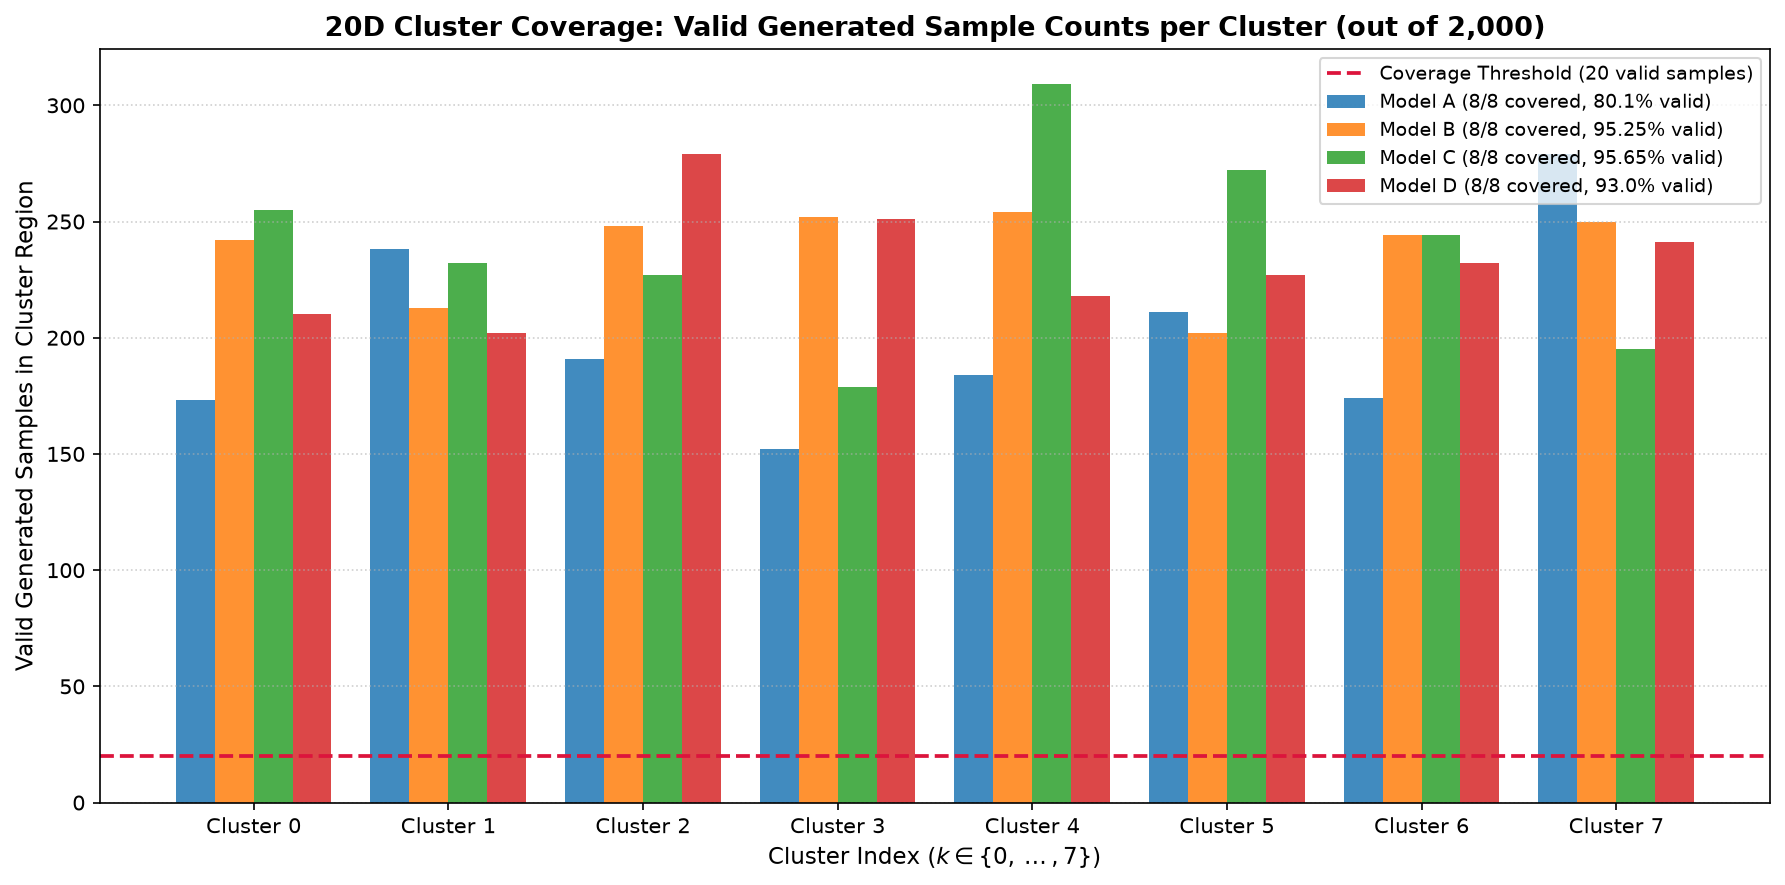
\includegraphics[width=0.75\linewidth]{problems/question2/results/cluster_coverage_comparison.png}
  \caption{مقایسه تفکیکی نرخ اعتبار کلی و توزیع نمونه‌های معتبر در هر یک از خوشه‌های ۸‌گانه در فضای ۲۰‌بعدی.}
  \label{fig:cluster-coverage}
\end{figure}

\textbf{پاسخ به سوال تحلیلی ۳ (مقایسه مدل C با ۸ مؤلفه و مدل D با ۴ مؤلفه):}
مطابق شکل~\ref{fig:cluster-coverage}، هر دو مدل شرط پوشش کامل (حداقل ۲۰ نمونه در تمام ۸ خوشه) را با موفقیت احراز کرده‌اند (مدل C در هر خوشه بین ۱۷۹ تا ۳۰۹ نمونه و مدل D بین ۲۰۲ تا ۲۷۹ نمونه معتبر تولید کرده‌اند). با این حال، مدل C به نرخ اعتبار $95.65\%$ در برابر $93.00\%$ مدل D می‌رسد. علت این است که مدل C ساختار توپولوژیک حقیقی تولید داده (۸ خوشه مدور) را منعکس می‌کند، در حالی که مدل D با ۴ مؤلفه مجبور است ساختار فضایی را فشرده کند که منجر به ایجاد نمونه‌های سرگردان در فضای بین‌خوشه‌ای می‌شود.

% =========================================================================
% ۵. تحلیل پژوهشی و جمع‌بندی
% =========================================================================
\subsection{تحلیل پژوهشی، مقایسه با VampPrior و جمع‌بندی}
\label{sec:q2-research}

\textbf{پاسخ به سوال تحلیلی ۵ (اثر سوگیری استقرایی مدل B در برابر مدل A):}
مدل B با بهره‌گیری از دانش صریح مسئله (۸ مؤلفه روی دایره‌ای به شعاع ۲) دارای یک سوگیری استقرایی (\lr{Inductive Bias}) قوی و منطبق بر حقیقت تولید داده است. این امر مانع از ایجاد چاله تهی در مرکز فضای نهفته شده و شکاف میان پسین تجمیعی $q(z) = \frac{1}{N}\sum q_\phi(z|x)$ و پیشین $p(z)$ را به حداقل می‌رساند که نتیجه آن کمترین مقدار $\text{MMD}^2$ هم در فضای داده ($0.00094$) و هم در فضای نهفته (مقدار بدون‌سوگیری ناچیز $-0.00037$) است.

\textbf{پاسخ به سوال تحلیلی ۶ (مقایسه پیشین یادگیرنده مدل C با پیشین ثابت مدل B):}
پیشین یادگیرنده به مدل این امکان را می‌دهد که موقعیت و پراکندگی خوشه‌ها را بر اساس پویایی آموزش بهینه‌سازی کند. مدل C با مراکز یادگرفته‌شده آزاد، به بالاترین نرخ اعتبار خوشه‌ای ($95.65\%$) در میان تمام مدل‌ها دست یافته است. با این حال، به دلیل انعطاف‌پذیری و آموزش همزمان پارامترهای پیشین و رمزگذار، خطای $\text{MMD}^2$ آن اندکی بالاتر از مدل B با مراکز متقارن ایده‌آل است.

\textbf{پاسخ به سوال تحلیلی ۷ (چرا ترکیب گاوسی یادگیرنده یک VampPrior نیست؟):}
روش \lr{VampPrior} (\cite{tomczak2018vampprior}) با پیشین ترکیب گاوسی یادگیرنده دارای تفاوت‌های ساختاری و ریاضی بنیادین زیر است:
\begin{enumerate}
  \item \textbf{فضای پارامتری و اتصال به شبکه:} در ترکیب گاوسی یادگیرنده، پارامترهای $(\mu_k, \sigma_k^2)$ متغیرهایی آزاد و مجزا در فضای نهفته دوبعدی هستند که مستقیماً در فضای نهفته بهینه‌سازی می‌شوند و هیچ پیوند ساختاری با شبکه رمزگذار ندارند. اما در \lr{VampPrior}، پیشین از طریق مجموعه‌ای از شبه‌ورودی‌های یادگیرنده (\lr{Pseudo-inputs}) $u_k \in \mathbb{R}^{D}$ در \textbf{فضای داده‌ها} تعریف می‌شود:
  \begin{equation}
    p(z) = \frac{1}{K}\sum_{k=1}^K q_\phi(z \mid u_k)
  \end{equation}
  \item \textbf{تقریب پسین تجمیعی (\lr{Aggregated Posterior}):} هدف ایده‌آل پیشین در VAE انطباق با پسین تجمیعی $q(z) = \int q_\phi(z|x)p_{\text{data}}(x)dx$ است. \lr{VampPrior} به طور مستقیم این پسین تجمیعی را با میانگین‌گیری روی نمایش رمزگذار از شبه‌داده‌های $u_k$ تقریب می‌زند، در حالی که پیشین ترکیب گاوسی معمولی نمی‌تواند به طور پویا با تغییرات وزن‌های رمزگذار $\phi$ همگام شود.
\end{enumerate}

\textbf{محدودیت‌ها و ملاحظات آزمایش:}
۱) کلیه آزمایش‌ها با یک بذر تصادفی ثابت اجرا شده‌اند؛ برآورد دقیق واریانس عملکرد نیازمند ارزیابی چندبذره است.
۲) مقدار منفی $\text{MMD}^2$ در مدل B ناشی از رفتار ذاتی برآوردگر آماری بدون‌سوگیری با واریانس محدود نمونه‌ای است و دلیلی بر برابری قطعی توزیع‌ها نیست.
۳) معیار اعتبار خوشه‌ای به مقدار آستانه صدک ۹۵ام محاسبه‌شده بر روی داده‌های اعتبارسنجی وابسته است.

\textbf{جمع‌بندی نهایی:} نتایج تجربی این پروژه به روشنی اثبات نمود که در داده‌های دارای چندگانگی و خوشه‌بندی طبیعی، جایگزینی پیشین گاوسی ساده با پیشین‌های غنی چندمدی (ثابت یا یادگیرنده) پدیده تولید نمونه‌های نامعتبر را برطرف کرده و وفاداری آماری نمونه‌های تولیدی را به طرز چشمگیری ارتقا می‌دهد.
